\begin{frame}
  \frametitle{Pervasive ``intelligent'' systems}
  \begin{columns}
    \begin{column}{0.3\textwidth}
      \centering
      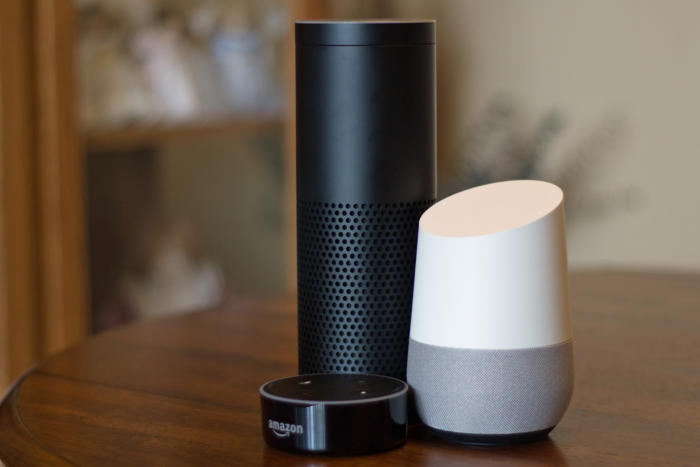
\includegraphics[width=\textwidth]{figures/echo-home.jpg}
      \\
      Home assistants

      \vspace{\fill}

      \bigskip

      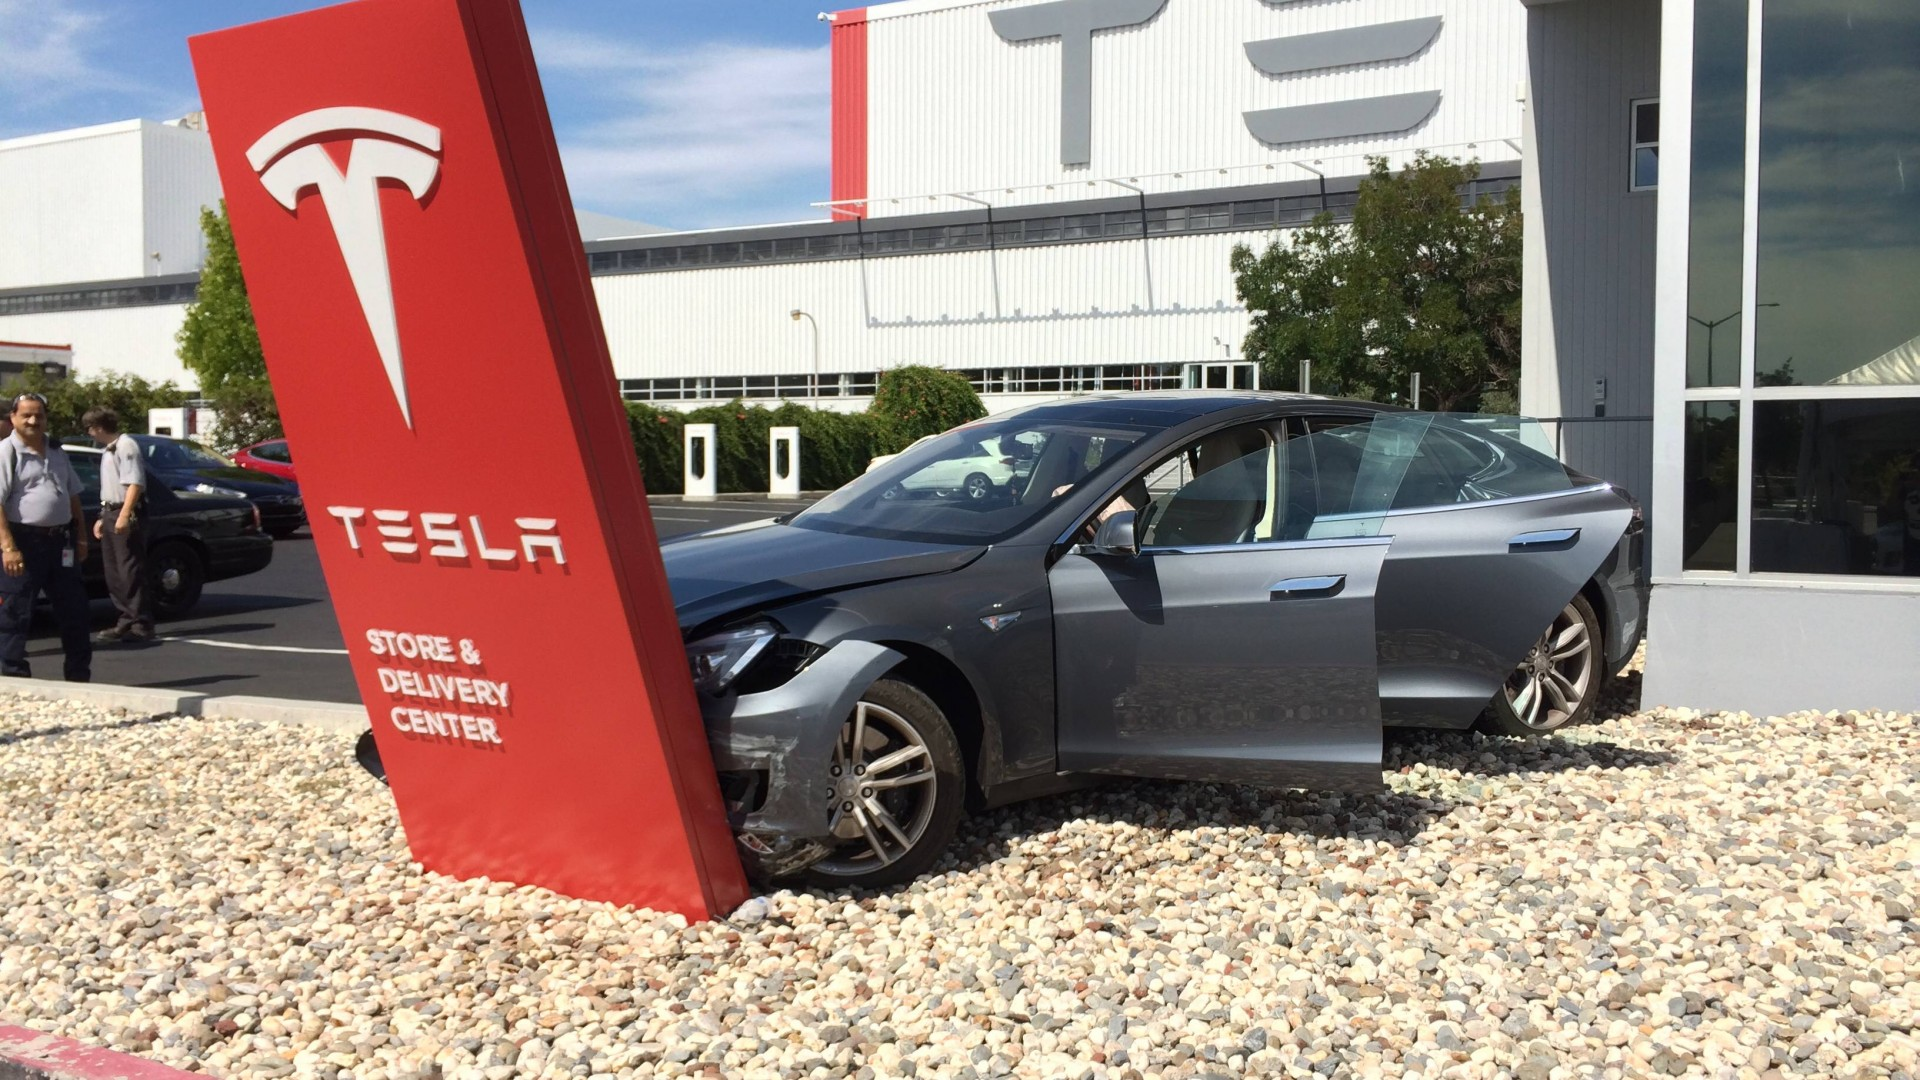
\includegraphics[width=\textwidth]{figures/tesla.jpg}
      \\
      Autonomous vehicles
    \end{column}
    \begin{column}{0.3\textwidth}
      \centering 
      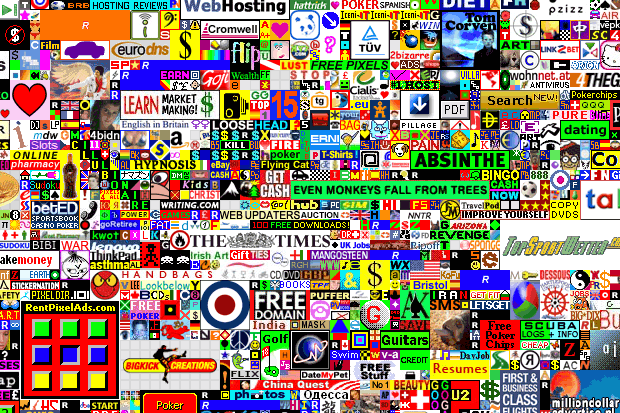
\includegraphics[width=\textwidth]{figures/web-ads.png}
      \\
      Web advertising

      \vspace{\fill}

      \bigskip

      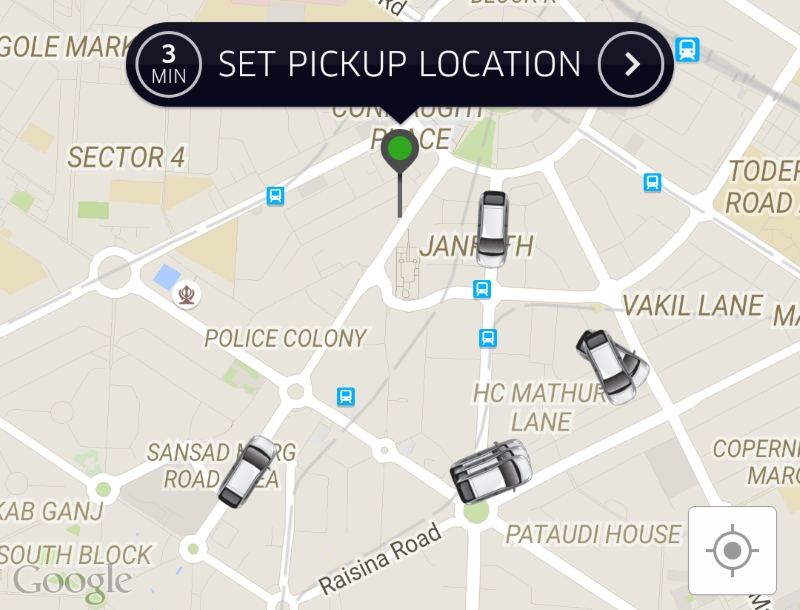
\includegraphics[width=\textwidth]{figures/uber-here-maps.jpg}
      \\
      Ridesharing
    \end{column}
    \begin{column}{0.3\textwidth}
      \centering 
      \\
      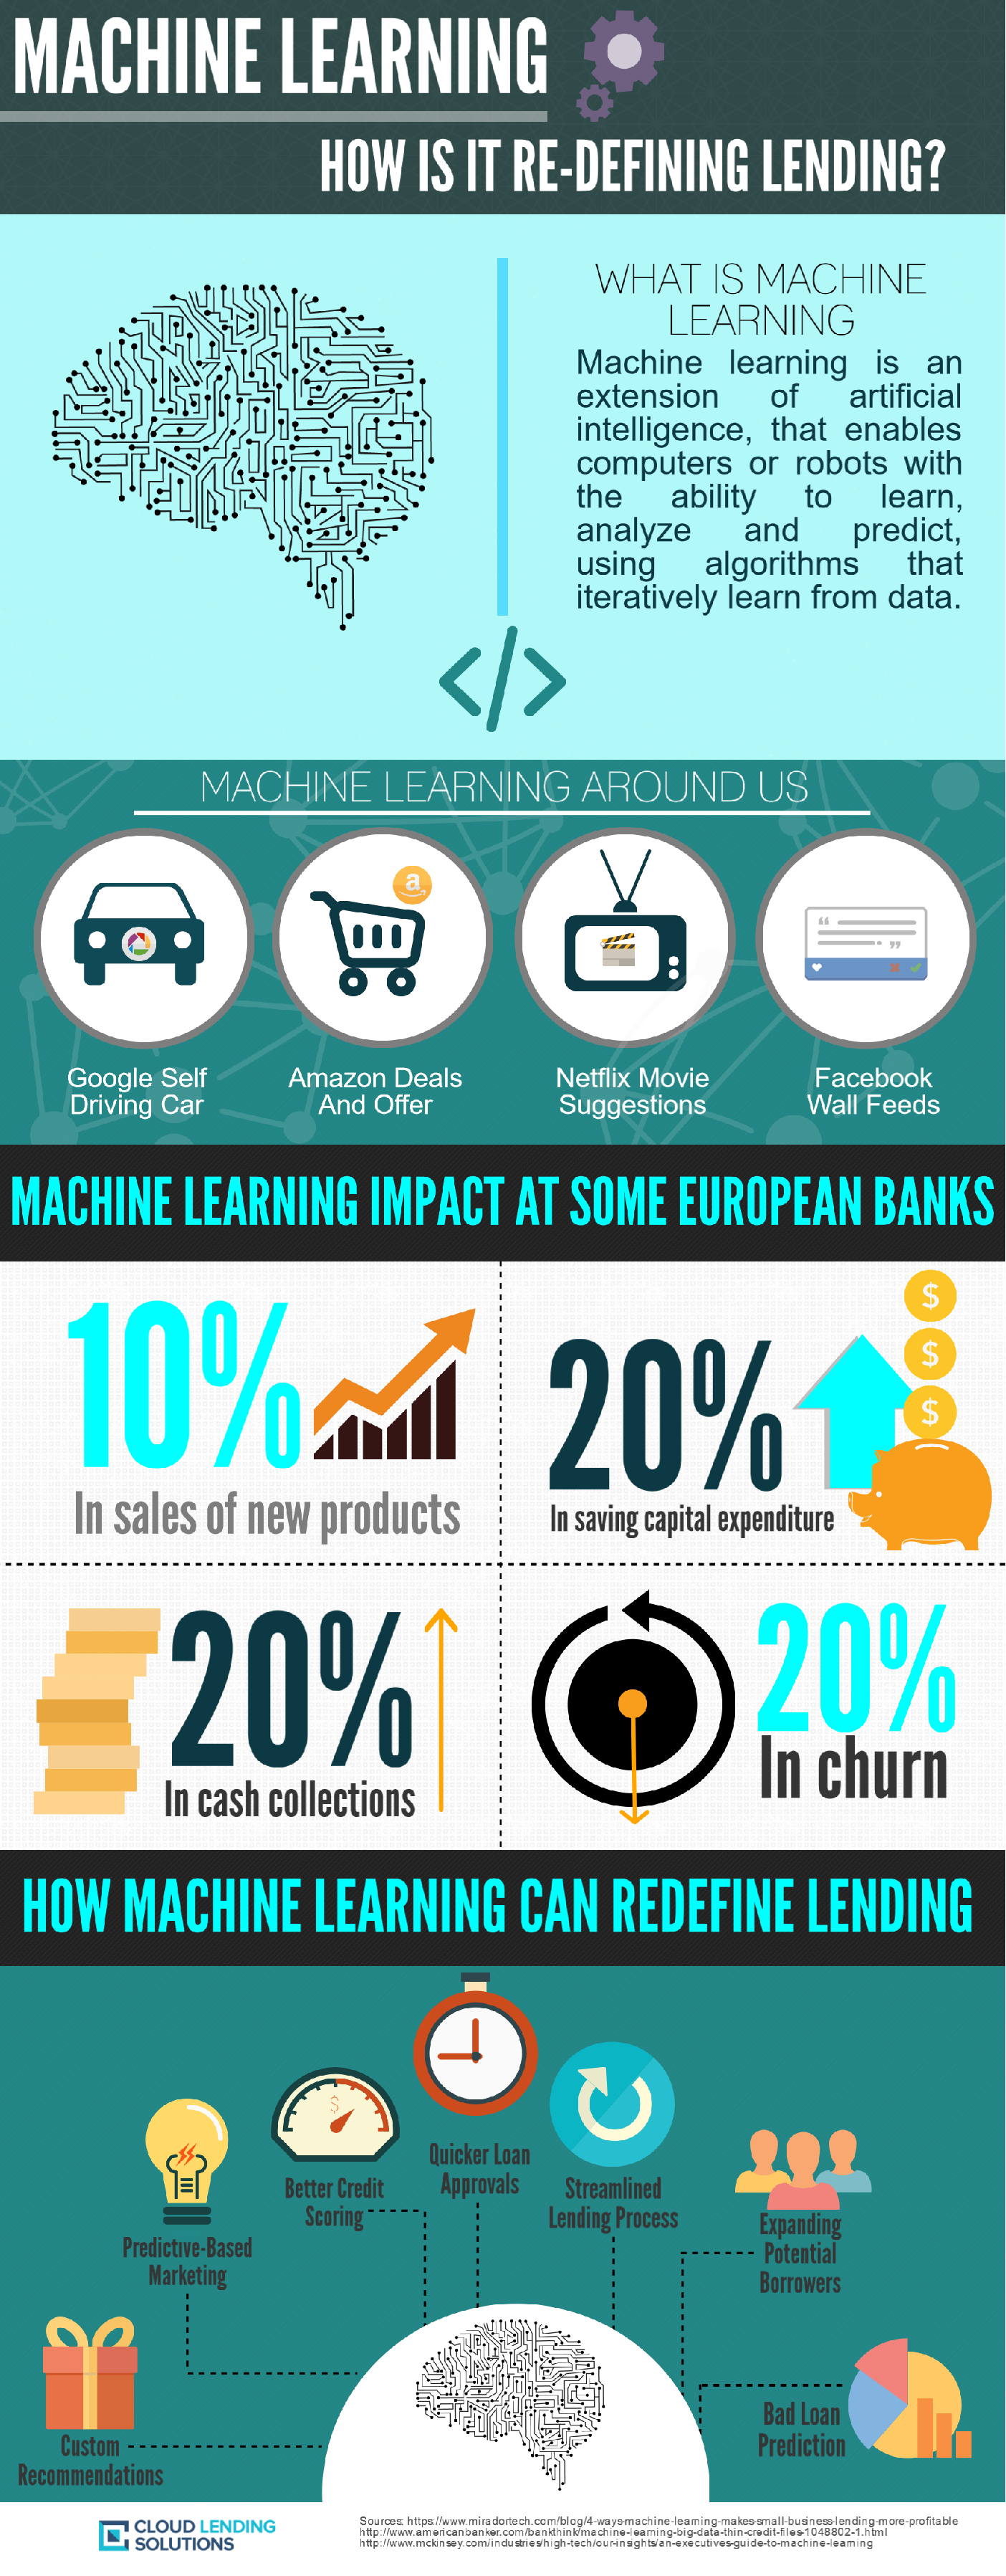
\includegraphics[width=\textwidth,clip = true, trim=0 0 0 42.5cm]{figures/lending.pdf}
      \\
      Lending

      \vspace{\fill}

      \bigskip

      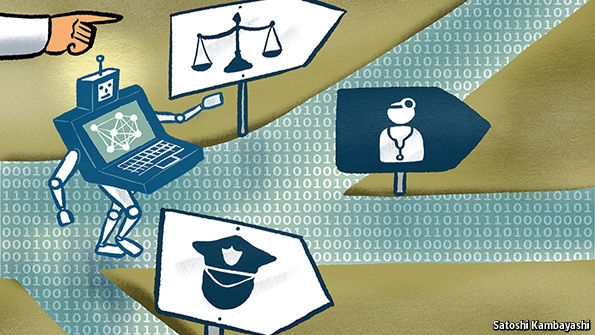
\includegraphics[width=\textwidth]{figures/algorithms-public.jpg}
      \\
      Public policy
    \end{column}
  \end{columns}
  \only<2>{
    \begin{tikzpicture}[remember picture,overlay]
      \draw[fill=black,opacity=0.75] 
      (current page.north east) rectangle (current page.south west);
      \node at (current page.center) {
        {\Huge \alert{Privacy, Fairness, Safety}}
      };
    \end{tikzpicture}}
  \pnote{Artificial intelligence is no longer limited to scientific applications and classical problems in AI such as playing games. AI is now deployed at large scale. These range from simple recommendation systems such as home assistants gather information about our habits, showering us with targeted ads and financial services; or more complex systems such as semi-autonomous vehicles. AI systems are also used increasing to direct human lives: ridesharing is an easy example, as drivers obtain instructions from an automated system. A less-known example is that AI now also shapes public policy. Automated policing, medical diagnostics and justice, are three cases in point.}
\pnote{Even if we assume these systems are well-designed, they have many negative implications. The first is privacy. In order to enable these technologies, some personal data must be collected. What guarantees do we have about how the data is used and what type of personal information can be leaked? The second is fairness. If a ridesharing app replaces standard taxis and buses, would this result in degraded transport services in poor areas of town? Would our CV screening application routinely turn down excellent female applicants? Finally, what can we say about the safety, i.e. the tail risks of technologies such as self-driving cars?}
\end{frame}

%%% Local Variables:
%%% mode: latex
%%% TeX-master: "basel-presentation"
%%% End:
